\section{Ablations and Negative Results}
\label{sec:negative-results}

\subsection{Missingness-aware FiLM}

The frozen-backbone static adapter improves ETTh1 random-0.3 MSE from 0.425394 to 0.361377. A missingness-aware FiLM adapter reaches 0.363156, which is 0.001778 worse than the static adapter. The mechanism audit finds a nonconstant condition representation, nonzero FiLM modulation, finite gradients, and updated conditioning parameters. These checks do not support an optimization or gradient-flow failure.

The supported interpretation is narrower: the tested global-statistics FiLM conditioning adds no generalization value beyond matched static capacity in this fixed condition. It does not rule out local temporal or channel-structured conditioning. Detailed adapter results are retained in Appendix~\ref{app:adapter}.

\subsection{Additive split conformal calibration}

The conformal experiment uses a strict raw-time selection and calibration split with a 479-row embargo. Native test intervals are already near their nominal targets, while the calibration segment is descriptively harder. The evaluated additive correction has a nonnegative quantile and can only expand intervals. In this setting, expansion moves native test intervals toward overcoverage, increases width, and worsens both absolute coverage error and interval score.

Figure~\ref{fig:conformal-tradeoff} displays the tradeoff. Mask-severity conditioning changes bin-specific quantiles but does not repair the aggregate result. A test-label shrinkage calculation is retained only as a counterfactual diagnosis and is not a valid calibrator. This finding is specific to the additive score, split, dataset, and missingness condition.

\begin{figure}[t]
    \centering
    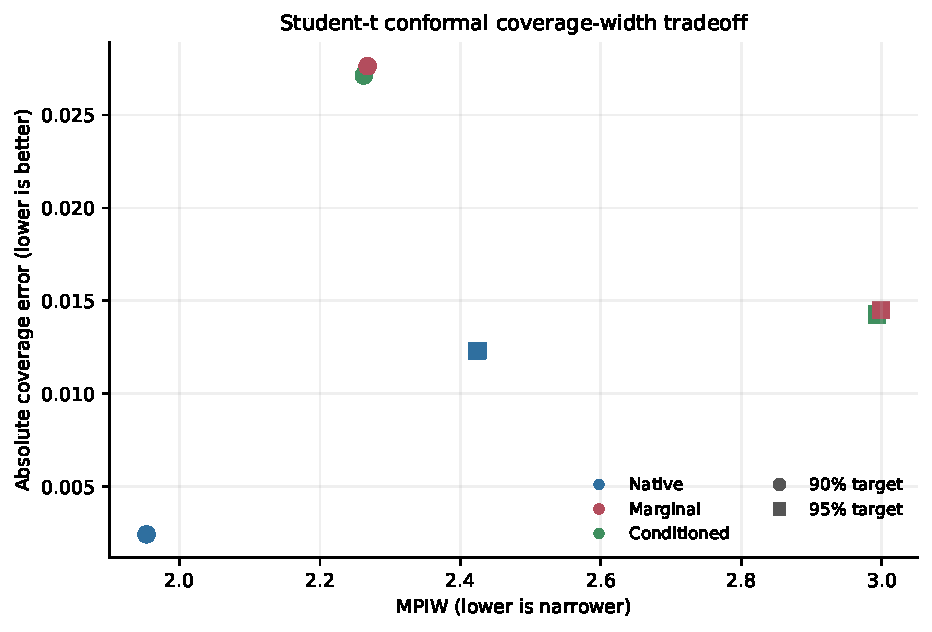
\includegraphics[width=0.88\linewidth]{figures/fig5_conformal_tradeoff.pdf}
    \caption{Native and additive conformal interval tradeoffs under the strict ETTh1 random-0.3 split. The additive procedures widen intervals without improving absolute coverage error.}
    \label{fig:conformal-tradeoff}
\end{figure}

\subsection{PatchTST point-prediction tradeoff}

The PatchTST Electricity result is not removed because its probabilistic scores improve. It is instead reported as a partial transfer result: NLL and CRPS improve, while relative MSE increases by 1.194\%. This single threshold miss changes the complete second-backbone decision from positive to a point-prediction tradeoff.
